\chapter{Rust for Networking Engineers}

This chapter adds a focused Rust primer tailored to building Smart Relay.

\section{Why Rust Here?}
\begin{itemize}
    \item Memory safety without GC pauses, good for long-lived daemons.
    \item Strong async ecosystem (Tokio, Axum) with first-class HTTP/QUIC support.
    \item Cross-platform builds let us target Windows/macOS/Linux with one codebase.
\end{itemize}

\section{Toolchain Quickstart}
\begin{itemize}
    \item Install Rustup, then \texttt{rustup target add x86\_64-pc-windows-msvc} etc.
    \item Project layout: \texttt{src/} for code, \texttt{Cargo.toml} for deps, \texttt{docs/} for this book.
    \item Build/test: \texttt{cargo build}, \texttt{cargo test}, run: \texttt{cargo run -- <args>}.
\end{itemize}

\section{Ownership and Borrowing in Practice}
\begin{itemize}
    \item Prefer \texttt{\&T} borrows for read-only config, \texttt{Arc<RwLock<T>>} when sharing mutable state across tasks.
    \item Avoid cloning large configs; use slices and references where possible.
\end{itemize}

\section{Async Primer (Tokio + Axum)}
\begin{figure}[h]
    \centering
    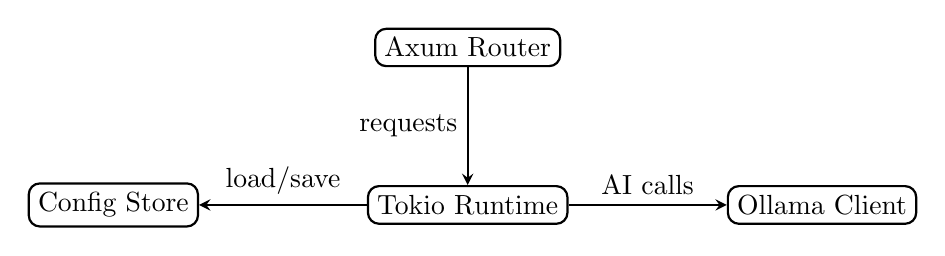
\begin{tikzpicture}[node distance=2cm,>=stealth,thick]
        \node (listener) [draw, rounded corners] {Axum Router};
        \node (runtime) [draw, rounded corners, below of=listener] {Tokio Runtime};
        \node (ai) [draw, rounded corners, right of=runtime, xshift=2.5cm] {Ollama Client};
        \node (cfg) [draw, rounded corners, left of=runtime, xshift=-2.5cm] {Config Store};
        \draw[->] (listener) -- node[left]{requests} (runtime);
        \draw[->] (runtime) -- node[above]{AI calls} (ai);
        \draw[->] (runtime) -- node[above]{load/save} (cfg);
    \end{tikzpicture}
    \caption{Axum handlers run inside the Tokio runtime, calling into AI and config subsystems asynchronously.}
\end{figure}

Minimal handler pattern:
\begin{verbatim}
#[derive(Deserialize)]
struct GoalBody { goal: Option<String> }

async fn propose(Json(body): Json<GoalBody>) -> Result<String, ApiError> {
    let goal = body.goal.unwrap_or("balanced".into());
    let plan = ai.propose_profile(&goal, Some(snapshot)).await?;
    Ok(plan)
}
\end{verbatim}

\section{Data Formats (Serde/TOML/JSON)}
\begin{itemize}
    \item Config persists to TOML via \texttt{serde} and \texttt{toml}.
    \item API responses use JSON automatically via Axum's \texttt{Json} extractor.
    \item Enable Serde features on external types (e.g., \texttt{uuid}).
\end{itemize}

\section{Error Handling}
\begin{itemize}
    \item Use \texttt{anyhow::Result} for binary entrypoints.
    \item Map errors to HTTP responses in handlers using a small helper (e.g., \texttt{internal\_error}).
    \item For library crates, prefer \texttt{thiserror} for typed errors.
\end{itemize}

\section{Testing Patterns}
\begin{itemize}
    \item Unit test prompt builders and config validators.
    \item Spin up Axum router with \texttt{tower::ServiceExt} for integration tests.
    \item Use \texttt{tokio::test} for async cases.
\end{itemize}

\section{Moving Forward}
After this primer, you should be comfortable reading the Smart Relay source, extending handlers, and integrating real proxy adapters.

